      \subsection{Nástroje pro replikaci v PostgreSQL}

PostgreSQL nabízí hned několik nástrojů pro řešení replikace. Je možno použít zabudovanou streaming replikaci, která je dostupná od verze PostgreSQL 9.0 nebo některou z extenzí, například Slony-I, pgpool, Skytools nebo Postgres-XC. Tato kapitola se dále bude zabývat a porovnávat nativní streaming replikace s extenzí Slony-I a pgpool.

      \subsubsection{Slony-I}
      \label{kSlony}

Jak píší \cite{Boszormenyi2013} je Slony-I jeden z nejrozšířenějších externích nástrojů pro replikaci pro PostgreSQL. Zároveň se také řadí mezi nejstarší, plně používán je v PostgreSQL již od verze 7.3. a je velmi dobře podporován i dalšími externími řešeními pro PostgreSQL, například programem PgAdmin3, který nabízí správu dat pomocí grafického rozhraní \citep{Boszormenyi2013}.

Jedná se o trigger-based replikaci, což znamená, že je ke každé exitující tabulce přidán trigger, který zajistí replikaci každé změny, která v databázi nastane. Z toho také vyplývá, že se jedná o logickou replikaci, kdy je možné replikovat pouze změny v datech, tzv. DDL změny, tedy SQL příkazy INSERT a UPDATE, nikoli strukturu databáze, příkazy typu CREATE/DROP TABLE, ALTER TABLE. Každá změna struktury se tedy musí provést ručně, což se může jevit jako nevýhodné. Nese to ale i své klady, například možnost výběru pouze některých tabulek. Vytváří si totiž tzv. replikační set, do kterého se zapíší pouze ty tabulky, které je potřeba replikovat. 

Další výhodou, a to zvlášť v porování se streaming replikací, je možnost replikace dat mezi různými verzemi PostgreSQL bez ohledu na platformu a architekturu. Naopak spíše za nevýhodu je považováno, že si vytváři ke každé tabulce vlastní schéma, do kterého se ukládají replikovaná data, což způsobuje redundanci dat. 

Slony-I replikace je z principu asynchronní, zpoždění je v řádu vteřin nebo v desítkách. Umožňuje Hot Standby mode, kdy je možno použít repliku na dotazy, i kaskádovou replikaci. Slony-I má vlastní konfigurační nástroj a samotná replikace funguje díky vlastnímu replikačnímu démonu, který běží stále, registruje změny a kopíruje je na slave servery.

      \subsubsection{Streaming replikace}
      \label{kStreaming}

Streaming replikace je nativní řešení do PostgreSQL implementováno od verze 9.0. Jedná se o log-shipping replikaci, což znamená, že jsou změny zapsány nejdříve vždy do transakčního logu v PostgreSQL nazvaného WAL (Write Ahead Log) přímým zápisem na disk a až poté potvzeny jako úspěšné. Tento způsob zajišťuje datům naprosté bezpeční, protože kdyby došlo k chybě a změny se nezapisovaly na disk, ale pouze do cache, mohlo by dojít k jejich ztrátě. Zároveň to zajišťuje kopii jak dat, tak i struktury databáze. Existuje pouze jeden transakční log pro jednu instalaci PostgreSQL, proto se replikují vždy všechny databáze a není možné výběru jen několika tabulek, tak jako u Slony-I \citep{Boszormenyi2013}. Protože replikace probíhá pomocí transakčního logu, je nutné použití stejné verze PostgreSQL, stejné platformy i architektury na všech uzlech replikačního clusteru. 

Streaming replikace umožňuje jak synchronní, tak asynchronní replikaci, dále Hot standby mode i kaskádovou replikaci.

      \subsubsection{pgpool}
      \label{kpgpool}
Nástroj pgpool, který je stejně jako Slony-I extenzí pro PostgreSQL, je dalším z nástrojů, které je možno v použít pro replikaci dat, umožňuje však i mnohé další funkce. Je prostředníkem pro komunikaci mezi klientem a PostgreSQL serverem a jeho hlavní úlohou je zvýšení efektivity a rychlosti práce s databází. 

Jednou ze základních výhod použití pgpool je možnost sdílení spojení klienta s databází, což v praxi znamená, že se vytvoří několik spojení, která i po skončení dotazu zůstanou otevřená a připravená pro další použití. Nemusí se tedy navazovat spojení při každém požadavku, ze strany klienta, což velice zrychlí provoz a zajistí plynulost užívání databáze. Umožňuje také paralerní dotazování, tedy složitý dotaz rozdělí mezi více uzlů, což velice sníží čas vykonání daného dotazu. 

Zároveň je nástrojem pro optimalizaci nastavení replikace, která je potřebná hned z několika důvodů \citep{pgpool2014}. V případě, že by v replikačním clusteru bylo třeba deset různých serverů, aby nedošlo k přetíže, bylo by nutné dát každému uživateli přístup k jinému serveru, nebo přístupy do databáze manuálně rozkládat skrze složité programové řešení. pgpool tohle vše zajišťuje sám. Navenek se jeví jako jakákoliv jiná databáze, do které se připojí všichni uživatelé bez ohledu na jejich práva či požadavky. On poté rozděluje dotazy mezi uzly v replikačním clusteru dle aktuální zátěže \citep{Boszormenyi2013}. Zároveň, pokud má uživatel přístup k zápisu i čtení, umí na základě jeho aktuálního SQL příkazu, rozhodnout, zda jej připojí k master nebo slave databázi, \odkazObrazek{pgpool-obr}. Tento způsob velmi zjednoduší jak administraci databáze, tak nastavení pro běžného uživatele, který se připojí pouze do jedné databáze a víc se nestará, zda z databáze pouze čte, nebo do ní i zapisuje. 
      \begin{figure}[H]
        \centering
        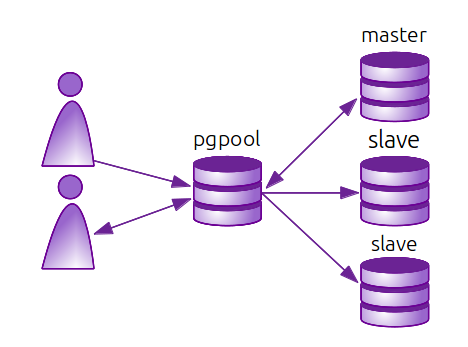
\includegraphics[scale=1]{../../../grafy/obr/schema_pgpool.png}
        \caption{Schéma pgpool}
        \label{opgpool}
      \end{figure}

